\subsubsection{Einstellen von Wirk- und Blindleistung}


$S = U*I, U=const$
P abgelesen
$Q = \sqrt{(S^2 - P^2)}$
\begin{figure}[!ht]
  \begin{center}
  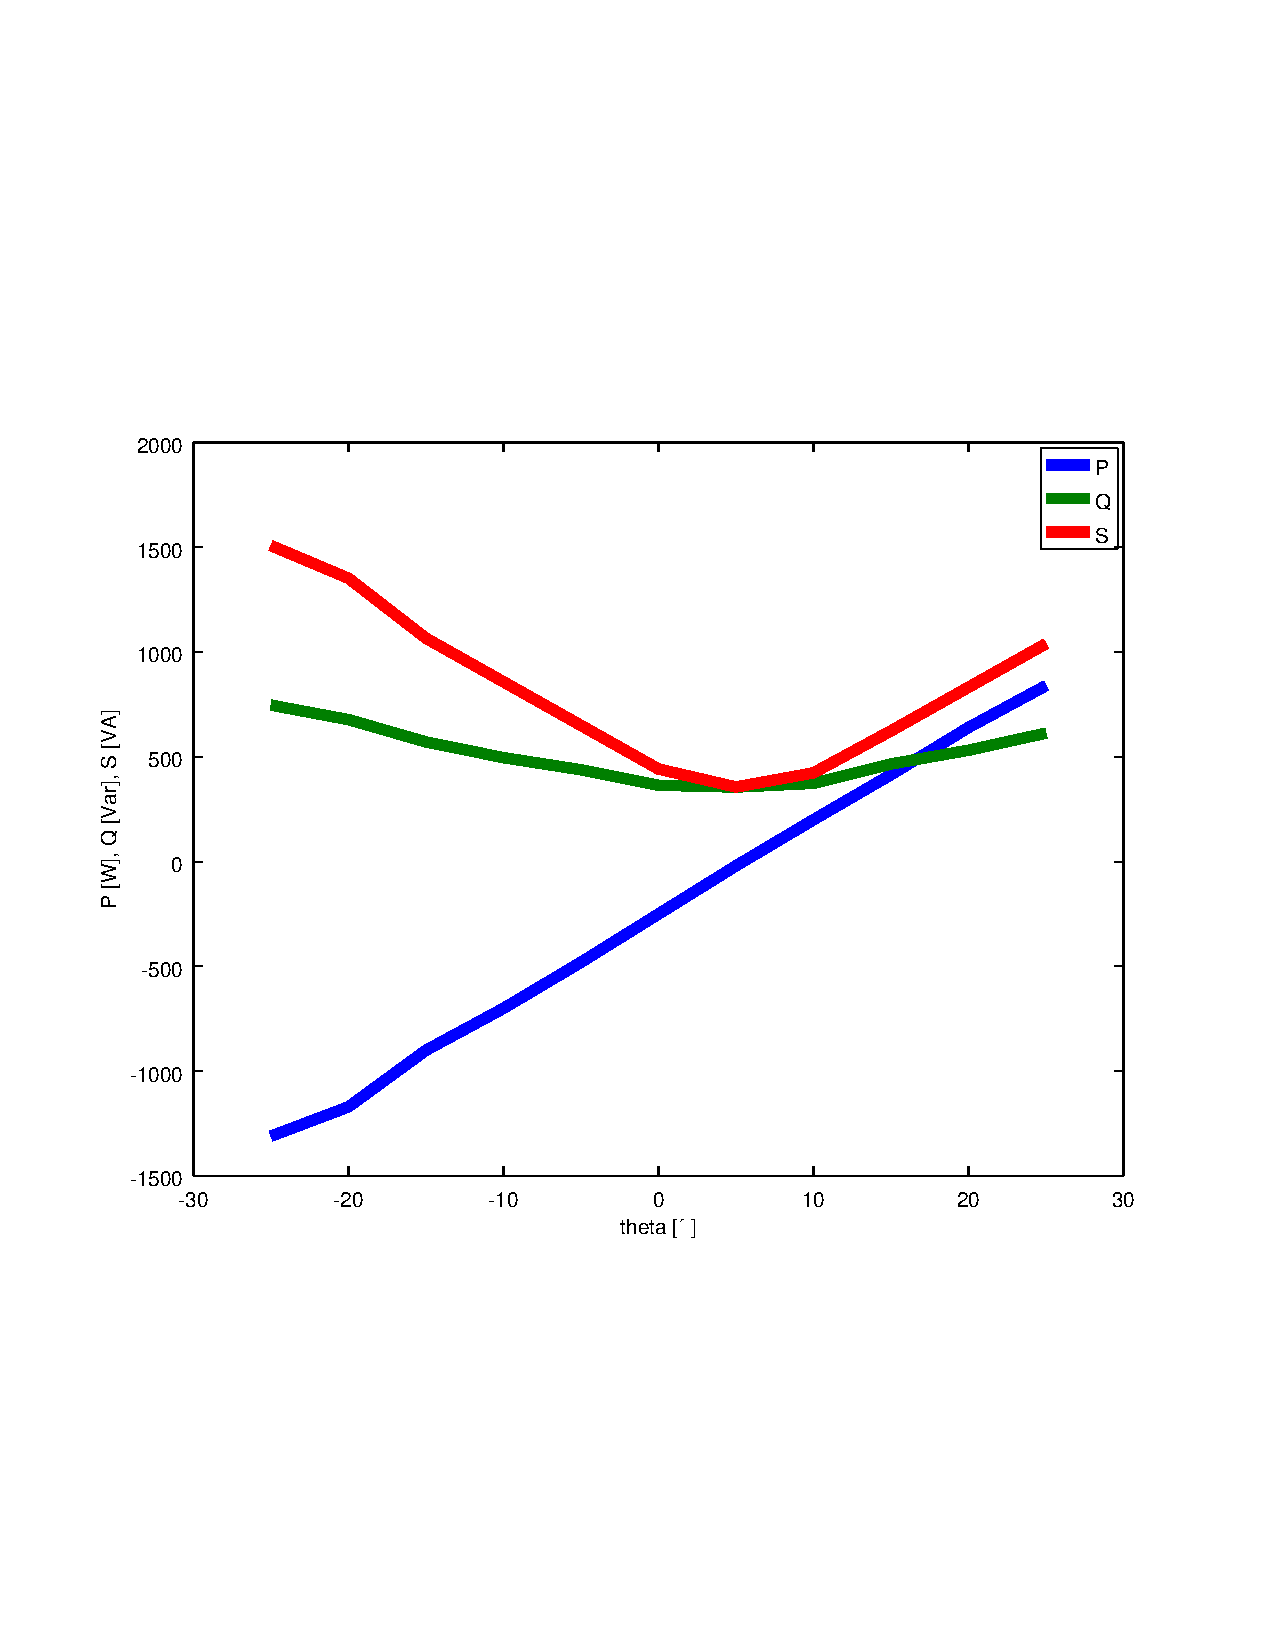
\includegraphics[width=0.5\textwidth, trim={1cm 6.5cm 2cm 7cm},clip]{pic/6_1_grundfrequenztaktung/6_1_2_einst_wirk_und_blindleistung/P_Q_S.pdf}
  \caption{P Q S}
  \label{fig:6_1_2_0}
  \end{center}
\end{figure}



$S_1 = U_1 * I_1$
\underline{I1} abgelesen, Trigger auf Strom
$P_1 = S_1 * cos(\phi)$
$Q_1 = S_1 * sin(\phi)$
\begin{figure}[!ht]
  \begin{center}
  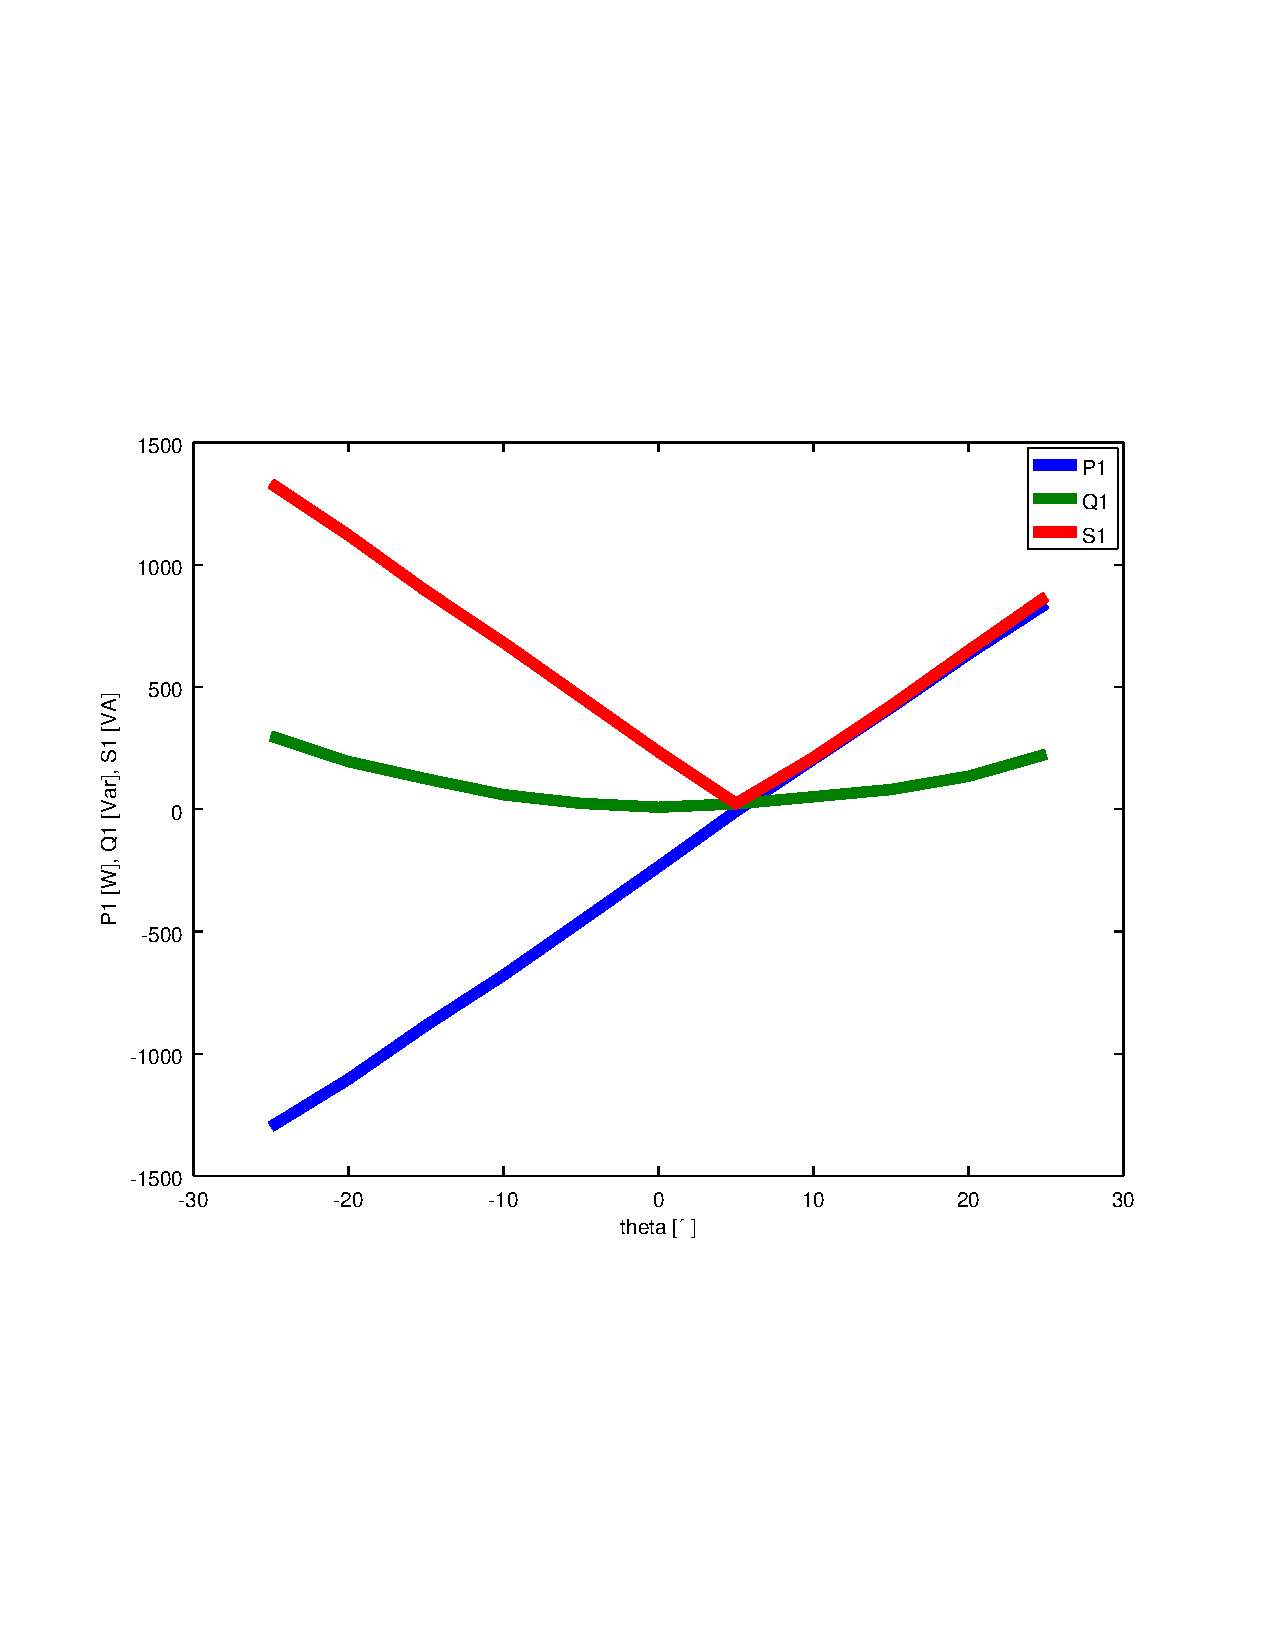
\includegraphics[width=0.5\textwidth, trim={1cm 6.5cm 2cm 7cm},clip]{pic/6_1_grundfrequenztaktung/6_1_2_einst_wirk_und_blindleistung/P1_Q1_S1.pdf}
  \caption{P1 Q1 S1}
  \label{fig:6_1_2_1}
  \end{center}
\end{figure}


Anhand von obigen Daten.
\begin{figure}[!ht]
  \begin{center}
  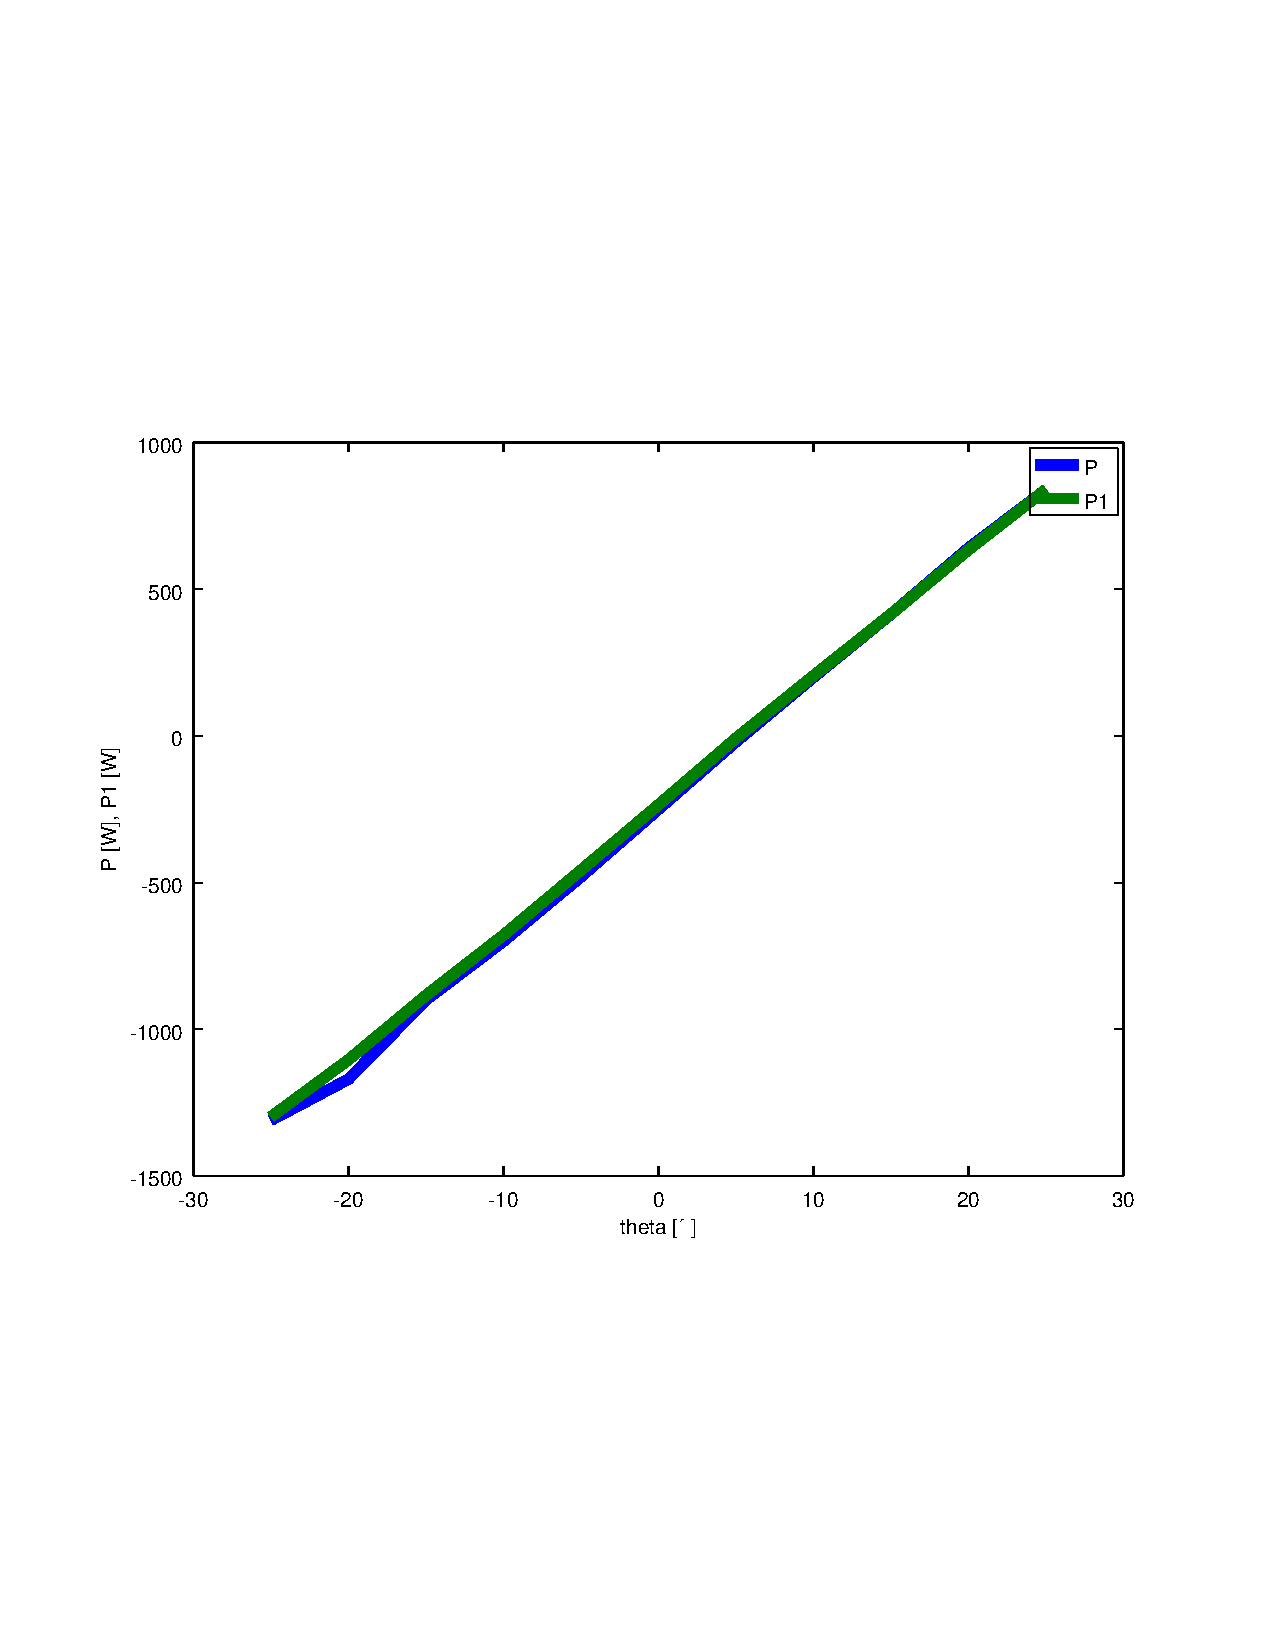
\includegraphics[width=0.5\textwidth, trim={1cm 6.5cm 2cm 7cm},clip]{pic/6_1_grundfrequenztaktung/6_1_2_einst_wirk_und_blindleistung/P_P1.pdf}
  \caption{P P1}
  \label{fig:6_1_2_2}
  \end{center}
\end{figure}


Anhand von obigen Daten.
\begin{figure}[!ht]
  \begin{center}
  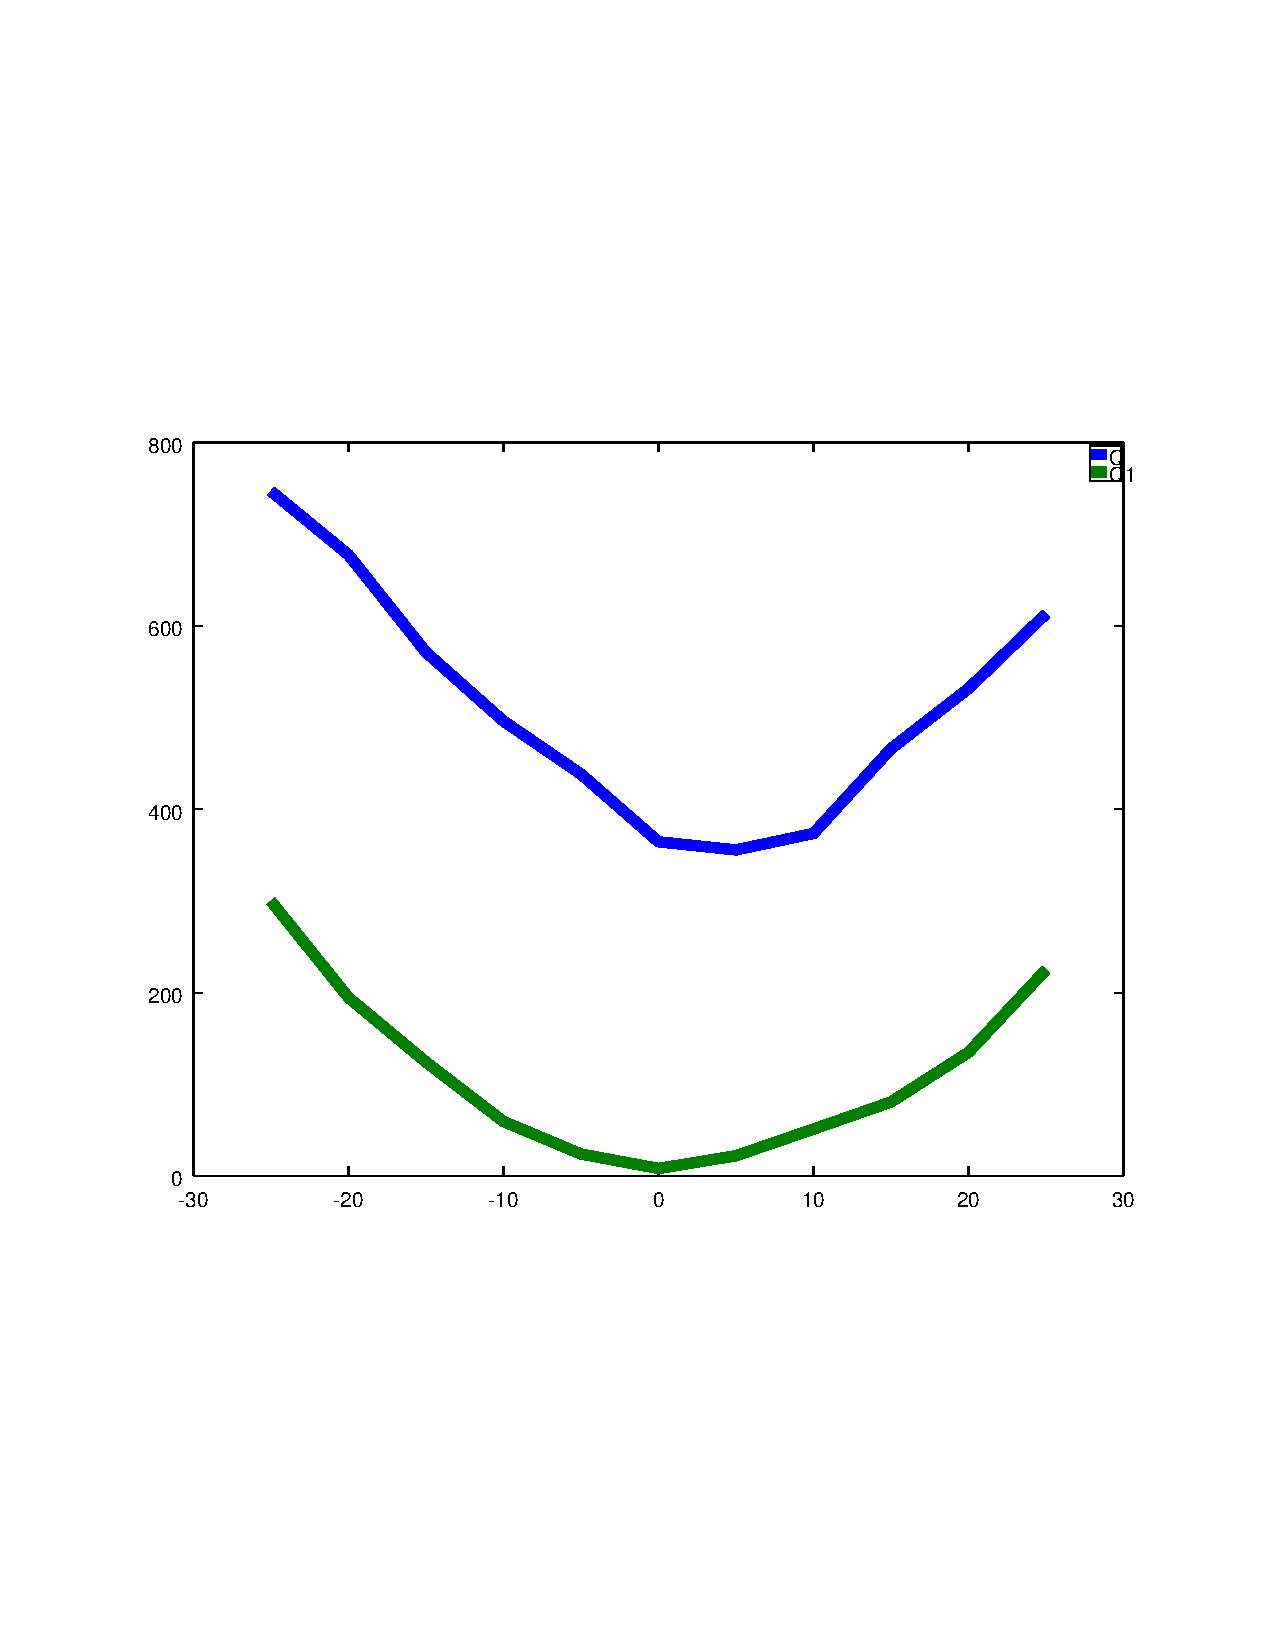
\includegraphics[width=0.5\textwidth, trim={1cm 6.5cm 2cm 7cm},clip]{pic/6_1_grundfrequenztaktung/6_1_2_einst_wirk_und_blindleistung/Q_Q1.pdf}
  \caption{Q Q1}
  \label{fig:6_1_2_3}
  \end{center}
\end{figure}



\clearpage